\newpage
\thispagestyle{empty}
\section{Gradientenverfahren}\label{sec:gradientenverfahren}   
\begin{tcolorbox}[title={Inhalte des \textit{Gradientenverfahren}}]
  \begin{quotation}\noindent
    Um die Verlustfunktion zu minimieren gibt es verschiedene Optimierungsverfahren. Das wohl bekannteste und am häufigsten eingesetzte Verfahren wird als Gradientenverfahren (Gradient Descent) bezeichnet.
    Das Kapitel Gradientenverfahren stellt die Grundlagen dar, die für das Verständnis des Lernprozesses eines neuronalen Netzwerks im nachfolgenden Kapitel erforderlich sind.
  \end{quotation}
  \begin{itemize}
    \item Wofür braucht man das Gradientenverfahren?
    \item Grundkonzepte des Gradientenabstiegsverfahren
    \item Gefährliche Fehlerquellen

  \end{itemize}
\end{tcolorbox}


\subsection{Wofür braucht man das Gradientenverfahren?}\label{subsec:gradientenverfahren:wofuer}
Das Gradientenverfahren (engl. gradient descent) wird genutzt, um ein Minimum einer Funktion mit beliebig vielen Parametern / Dimensionen zu finden.
Natürlich könnte man nun denken, dass man dies durch bereits bekannte Methoden auch algebraisch berechnen könnte, jedoch wird dies 
bei einer Funktion mit tausenden oder mehr Parametern sehr schwierig oder gar unmöglich.
Für neuronale Netze nutzt man das Gradientenverfahren konkret um ein Minimum der Verlustfunktion zu bestimmen. Durch diese Berechnung lässt sich mithilfe der Backpropagation jedes einzelne Gewicht und jeder Bias-Wert anpassen, hierdurch "lernt" das neuronale Netz.

\iffalse
\subsubsection{Was ist der Gradient einer Funktion?}\label{subsec:gradientenverfahren:was_ist_gradient}
  Ein Gradient ist eine Vektorfunktion, bestehend aus den partiellen Ableitungen der Funktion.
  Dieser beschreibt immer die Richtung der größten (steilsten) Steigung in einem Punkt p in Form eines Vektors.\cite{LH21}
  \\
  \\ Allgemein ist der Gradient einer Stelle $x^k$ für den k-ten Iterationsschritt wie folgt über die partiellen Ableitungen definiert:
  \\ $\operatorname{Grad}(f)(x^{(k)}) := \left(\frac{\partial f}{\partial x_{1}}(x^{(k)}), \cdots, \frac{\partial f}{\partial x_{n}}(x^{(k)})\right)$
  \\
  \\Hierbei sind $\frac{\partial f}{\partial x_{1}}(x^{(k)}), \dots, \frac{\partial f}{\partial x_{n}}(x^{(k)})$ die partiellen Ableitungen von f nach den einzelnen Variablen $x_{1}, \ldots, x_{n}$ an der Stelle $x^{(k)}$.
  Die partiellen Ableitungen messen die Veränderungsrate von f in Bezug auf jede einzelne Variable an der spezifischen Stelle $x^{(k)}$. Der Gradient ist dann ein Vektor, der diese Veränderungsraten in jeder Dimension repräsentiert.
  Die Formel definiert also den Gradienten als einen Vektor, der aus den partiellen Ableitungen der Funktion f nach den einzelnen Variablen besteht, evaluiert an der Stelle $x^{(k)}$.
\fi
\subsubsection{Was ist der Gradient einer Funtkion?}\label{subsec:gradientenverfahren:was_ist_gradient}
  Der Gradient einer Funktion $f(x_{1}, x_{2}, ... , x_{n})$ ist definiert durch die Funktion $\nabla f(x_{0})$, welche den Spaltenvektor $V$ liefert, in welchem jede Komponente $v_1$ bis $v_n$ die partielle Ableitung der Funktion $f$ nach dem jeweiligen Parameter 
  $x_{i}$ an der Stelle $x_0$ darstellt. Konkret also: 
  \renewcommand{\arraystretch}{1.5}
  \begin{align*}
    \nabla f(x_0) =\begin{bmatrix}
          \frac{\partial f}{\partial x_{1}}(x_{0}) \\
          \frac{\partial f}{\partial x_{2}}(x_{0}) \\
           \vdots \\
           \frac{\partial f}{\partial x_{n}}(x_{0}) \\
         \end{bmatrix}
  \end{align*}
  \renewcommand{\arraystretch}{1}
  Der Gradient an einem Punkt zeigt die Richtung des steilsten Anstiegs der Funktion an diesem Punkt an. Das bedeutet, dass,
  wenn man in die Richtung des Gradienten geht, man die Funktion so schnell wie möglich erhöht, und wenn man in die entgegengesetzte Richtung geht,
  also in Richtung des negativen Gradienten, man die Funktion so schnell wie möglich verringert. Dies ist ein entscheidender Aspekt bei dem Gradientenverfahren.
  \bigbreak\noindent
  Im folgenden wird der Gradient einer Funktion an einem simplen Beispiel berechnet: 
  \bigbreak\noindent
  Sei $f(x, y) = x^2 + y^2$, nun ist der Gradient für den Punkt $x = 5, y = 3$ gesucht. Es gilt
  \begin{align*}
    \frac{\partial f}{\partial x}(x,y) = f_{x}(x,y) = 2x\\
    \\
    \frac{\partial f}{\partial y}(x,y) = f_{y}(x,y) = 2y\\
  \end{align*}
  Somit ergibt sich für unsere Funktion $f$ folgender Gradient für den Punkt $x = 5, y = 3$ 
  \begin{align*}
    \nabla f(5, 3) = \begin{bmatrix}
      2 * 5\\
      2 * 3\\
    \end{bmatrix} = \begin{bmatrix}
      10\\
      6\\
    \end{bmatrix}
  \end{align*}

\subsection{Grundkonzepte des Gradientenverfahrens}\label{subsec:gradientenverfahren:grundkonzepte}

\iffalse
\subsubsection{Grundlage für den Fehlerrückführungs-Algorithmus - Wozu dient das Gradientenverfahren?}\label{subsec:gradientenverfahren:grundlage_fehlerrueckfuehrungsalg}
  Warum sollte das Minimum der Verlustfunktion gefunden werden? Das spätere Lernen geschieht durch Anpassung der Gewichte, es wird die Differenz aus der tatsächlichen und der korrekten Ausgabe bestimmt. 
  Schnell kann hier natürlich die Frage aufkommen, warum nähert man sich dem Minimum an und berechnen es nicht. Die Berechnung würde auf das Problem stoßen, dass es unendlich viele Richtungen gibt, in der die Funktion minimal werden könnte. 

  Das Backpropagation-Verfahren ist eine Möglichkeit den Gradientenabstieg anzuwenden. Auf die Fehlerbestimmung wird in Kapitel 4 - Backpropagation eingegangen. Der Gradientenabstieg liefert also die Grundlage, später das NN zu trainieren.

\fi

\subsubsection{Wie funktioniert das Gradientenverfahren?}\label{subsec:gradientenverfahren:wie_funktioniert}
  Das Gradientenverfahren ist ein iteratives Verfahren, bei welchem man sich in jedem Iterationsschritt immer näher in die Richtung des
  steilsten Abstiegs einer Funktion $f(x_{1}, x_{2}, ... , x_{n})$ bewegt. Somit nähert man sich nach einigen Iterationen zuverlässig einem Minimum der Funktion $f$ an.
  \bigbreak\noindent
  Wie bereits oben erwähnt, gibt uns der Gradientenvektor $\nabla f(x_{0})$ einer Funktion $f(x_{1}, x_{2}, ... , x_{n})$ die Richtung des steilsten Anstieges vom Punkt $x_0$ aus gesehen.
  Passen wir also jeden Parameter $x_{i}$ um den durch den Gradientenvektor gegebenen Wert $v_{i}$ an, bewegen wir uns damit weiter in Richtung des steilsten Anstieges. 
  Da wir uns beim Gradientenverfahren aber für das Minimum einer Funktion interessieren, geht man stattdessen in die entgegengesetzte Richtung
  des Gradientenvektors $-\nabla f(x_{0})$, also die Richtung des steilsten Abstiegs. Der Gradientenvektor gibt jedoch nicht, an wie weit man in die Richtung des steilsten 
  Abstiegs gehen sollte. Um also zu verhindern, dass man das Minimum "überschreitet" moderiert man die Schrittweite durch eine sogenannte Lernrate $\eta$.
  Der Startpunkt $x_{0}$ muss außerdem zu Beginn des Gradientenverfahrens zufällig ausgewählt werden.
  Damit haben wir die Grundidee des Gradientenverfahrens: 
  \begin{align*}
    \begin{bmatrix}
          x_{1}\\
          x_{2}\\
          \vdots \\
          x_{n}
         \end{bmatrix}_{Neu} = \begin{bmatrix}
          x_{1}\\
          x_{2}\\
          \vdots \\
          x_{n}
         \end{bmatrix}_{Alt} - \eta \nabla f(x_{0})
  \end{align*}
  \noindent
  Die Schritte des Gradientenverfahres sind also folgende: 
  \begin{enumerate}
    \item Auswahl eines zufälligen Startpunktes / Startparameter $x_{0}$
    \item Berechnen des Gradientenvektors $\nabla f(x_{0})$
    \item Anpassen der Startparameter durch den negativen Gradientenvektor multipliziert mit der Lernrate
  \end{enumerate}
  \bigbreak\noindent
  Die Schritte 2. und 3. wiederholt man nun eine feste Anzahl an Iterationsschritten, oder bis die Ursprungsfunktion $f$ gegen einen Wert konvergiert.
  \bigbreak\noindent
  Im Folgenden wird das Gradientenverfahren an einem konkreten Beispiel erläutert.
  Sei $f(x,y) = 3x^2 + 6y^2$ und ein zufällig ausgewählter Startpunkt $x = 3$ und $y = 4$. 
  Die Lernrate setzen wir auf $\eta = 0.05$. Dann berechnet sich der Gradient $\nabla f(3,4)$ wiefolgt: 
  \begin{align*}
    \frac{\partial f}{\partial x}(x,y) = f_{x}(x,y) = 6x\\
    \\
    \frac{\partial f}{\partial y}(x,y) = f_{y}(x,y) = 12y\\
    \\
    \Rightarrow \nabla f(3,4) = \begin{bmatrix}
      6 * 3\\
      12 * 4\\
    \end{bmatrix} = \begin{bmatrix}
      18\\
      48\\
    \end{bmatrix}
  \end{align*}
  Nun passen wir die Startparameter gemäß der Vorschrift mithilfe des negativen Gradientenvektors multipliziert mit der Lernrate an: 
  \begin{align*}
    \begin{bmatrix}
      3\\
      4\\
    \end{bmatrix} - 0.05 * \begin{bmatrix}
      18\\
      48\\
    \end{bmatrix} = \begin{bmatrix}
      2.1\\
      1.6\\
    \end{bmatrix}
  \end{align*}
  Bereits jetzt ergibt sich ein erheblicher Unterschied, wohingegen $f(3,4) = 51$ ergibt, bekommen wir mit unseren aktualisierten Parametern bereits 
  $f(2.1, 1.6) = 28.59$. Wir nähern uns also einem Minimum an! Die weiteren Iterationsschritte sind nur noch in verkürzter Form angegeben:
  \begin{align*}
    \begin{bmatrix}
      2.1\\
      1.6\\
    \end{bmatrix} - 0.05 * \begin{bmatrix}
      6 * 2.1\\
      12 * 1.6\\
    \end{bmatrix} = \begin{bmatrix}
      1.47\\
      0.64\\
    \end{bmatrix} \Rightarrow f(1.47, 0.64) = 8.94
    \\\\
    \begin{bmatrix}
      1.47\\
      0.64\\
    \end{bmatrix} - 0.05 * \begin{bmatrix}
      6 * 1.47\\
      12 * 0.64\\
    \end{bmatrix} = \begin{bmatrix}
      1.02\\
      0.256\\
    \end{bmatrix} \Rightarrow f(1.02, 0.256) = 3.51
    \\\\
    \begin{bmatrix}
      1.02\\
      0.256\\
    \end{bmatrix} - 0.05 * \begin{bmatrix}
      6 * 1.02\\
      12 * 0.256\\
    \end{bmatrix} = \begin{bmatrix}
      0.714\\
      0.1024\\
    \end{bmatrix} \Rightarrow f(0.714, 0.1024) = 1.59
    \\\\
    \begin{bmatrix}
      0.714\\
      0.1024\\
    \end{bmatrix} - 0.05 * \begin{bmatrix}
      6 * 0.714\\
      12 * 0.1024\\
    \end{bmatrix} = \begin{bmatrix}
      0.5\\
      0.04\\
    \end{bmatrix} \Rightarrow f(0.5, 0.04) = 0.76
    \\\\
  \end{align*}
  Wie man sieht nähern sich unsere Funktionswerte mit jedem Iterationsschritt
  der 0. Würde man das Gradientenverfahren einige Iterationen weiter ausführen, so 
  würde man schlussendlich die Werte $x = 0$ und $y = 0$ rausbekommen. Dort liegt unser Minimum.
  \bigbreak\noindent
  Die Auswahl des Startpunktes $x_{0}$ sowie die Wahl der Lernrate $\eta$ spielen eine große Rolle beim Erfolg des
  Gradientenverfahrens, hierauf wird jedoch nicht weiter eingegangen.
\iffalse
\subsubsection{Wie funktioniert das Gradientenverfahren?}\label{subsec:gradientenverfahren:wie_funktioniert}
'Das Gradienten Verfahren (GV) ist ein iteratives Verfahren mit dem Ziel ein Minimum einer Funktion zu finden. Hierbei wird in jedem Schritt ein Stück in die Richtung des Gradienten
gegangen. Da wir an dem Minimum der Funktion interessiert sind, bedeutet das für den Algorithmus, dass wir in die negative Richtung des Gradienten gehen müssen'\cite{LH21}[Seite 9].
\\
Im Fall von künstlichen neuronalen Netzen suchen wir das Mimimum der Verlustfunktion und wollen diesem sehr schnell nahe kommen.
Wenn wir also in die negative Richtung des Gradienten gehen, wissen wir, dass die Funktion am stärksten abfällt und wir somit auch dem Minimum am schnellsten näher kommen. Das Verfahren durchläuft folgende Schritte:
  \begin{itemize}
    \item Wahl eines (zufälligen) Startpunktes
  \end{itemize}
  \begin{itemize}
    \item Festsetzung eines Lernparameters
  \end{itemize}
  \begin{itemize}
    \item Festlegung des Abbruchkriterium
    \begin{itemize}
    \item Fixierung der kritischen Differrenz der Gewichtsveränderungen, die nicht unterschritten werden darf
    \item Spezifizierung der maximalen Anzahl an Iterationen (Wiederholungen), die vorgenommen werden sollen.
    \end{itemize}
  \end{itemize}
  \begin{itemize}
    \item  Berechnung des Gradienten
  \end{itemize}
  \begin{itemize}
    \item Veränderung der Gewichte
  \end{itemize}

  %Wahl eines (zufälligen) Startpunktes
Das Gradientenverfahren generiert ausgehend von einem Startpunkt $x^0\epsilon\mathbb{R}^n$ eine Folge von Punkten $x^k\epsilon\mathbb{R}^n$ gemäß der Iterationsvorschrift $x^k+1=x^k+\alpha^k d^k, k=0,1,\dots$ 
  wobei $\alpha^k>0$ eine positive Schrittweite ist und $d^k\epsilon\mathbb{R}^n$ eine Abstiegsrichtung.
  \\ 
  Dabei werden sowohl $\alpha^k$ als auch $d^k$  in jedem Iterationsschritt so bestimmt, dass die Folge $x^k$ zu einem stattionären Punkt von $f$ konvergiert.
  %TO-DO Festsetzung eines Lernparameters
  %TO-DO Festlegung des Abbruchkriterium
  Eine Abbruchbedingung für das Gradientabstiegsverfahren wäre, wenn wir mit der Iteration eine Stelle $x^k\epsilon\mathbb{R}^n$ gefunden haben an der der Gradient von $f$gleich 0 ist, also
  $\text{Grad}(f)(x^{(k)}) = 0 \in \mathbb{R}^n$
  %TO-DO Fixierung der kritischen Differrenz der Gewichtsveränderungen, die nicht unterschritten werden darf. Spezifizierung der maximalen Anzahl an Iterationen (Wiederholungen), die vorgenommen werden sollen.
  %TO-DO Berechnung des Gradienten
  \\
\newline Der Gradient ist ein Vektor der aus den partiellen Ableitungen der Komponenten einer Funktion besteht. Unsere Funktion hat zwei Komponenten: x und y.
  Das heißt der Gradient unserer Funktion ist ein Vektor mit Zwei Komponenten.
  Um die partielle Ableitung einer Komponente zu bilden betrachten wir alle Glieder der Formel in der diese Komponente vorkommt und leiten die ab. 
  \\Die partielle Ableitungen sind also:
  \\$f_x(x, y) = 2x + 2y - 6 \quad \text{und} \quad f_y(x, y) = 2x + 4y - 16$
  \\
  \\Damit sieht unser Gradient wie folgt aus:
  \newline $\nabla f(x, y) = (2x + 2y - 6, 2x + 4y - 16)$
  \\
  \\
  Nun bestimmen wir den Gradienten ausgehend von unserem Startpunkt P=(1,3). Also einfach den Punkt einsetzen. 
  \newline $\nabla f(1,3) = (2 \cdot 1 + 2 \cdot 3 - 6, 2 \cdot 1 + 4 \cdot 3 - 16) = (2 - 2)$
\\
\\
Bei einem normierten Gradienten beträgt die Länge exakt 1, da das in den meisten fällen nicht zutrifft müssen wir den Gradienten zu aller erst normieren bevor wir ihn für unsere Suchgerade verwenden können. Um einen Vektor auf die Länge 1 zu normieren wird er mittels Skalarmultiplikation mit seiner derzeitigen Länge dividiert. Logisch, wenn du eine Zahl durch sich selbst teilst kommst du immer auf 1 ;D
  Die Länge des Gradienten ermittelst du indem du den Betrag bildest, also:
  \newline $|\nabla f(1,3)| = \sqrt{2^2 + (-2)^2} \approx 2.83$
\\
\\
Nachdem du die Länge ermittelt hast heißt es nurnoch jede Komponente durch die Länge zu teilen:
  $||\nabla f(1,3)|| = \frac{2 - 2}{\sqrt{2}} \approx (0.707 - 0.707)$
\\
\newpage
Die Veränderung erfolt, indem die alten Gewichte um das Produkt aus Lernrate und Gradienten subtrahiert werden. Durch die Multiplikation mit der Lernrate kann die Größe der Aktualisierung gesteuert werden.
  Eine größere Lernrate führt zu größeren Aktualisierungen und möglicherweise schnellerer Konvergenz, birgt jedoch das Risiko des Overshootings und des Verfehlens des Minimums.
  Eine kleinere Lernrate führt zu kleineren Aktualisierungen und möglicherweise langsamerer Konvergenz, aber mit größerer Stabilität. 
Als Overshooting bezeichnet man die Situation, indem der Parameter über das gesuchte Minimum hinausschießt und sich von diesem entfernt.
Der vierte und der fünfte Punkt werden solange wiederholt, bis mindestens eines der beiden Abbruchkriterien erfüllt ist (siehe dritter Punkt).
  'Das Gradientenverfahren beginnt mit einer zufälligen Gewichtskombination, die die Startposition auf der Kurve bzw. in einer n-dimensionalen 'Gebirgslandschaft' makiert.
  Von dieser Position aus soll nun das 'tiefste Tal', in der 'Hügellandschaft' gesucht werden'\cite{GR10}.
  
\fi

\iffalse
\subsubsection{Mehrere Dimensionen}\label{subsec:gradientenverfahren:mehrere_dimensionen}
 Das Gradientenverfahren beginnt mit einer zufälligen Gewichtskombination, die die Startposition auf der Kurve bzw. in einer n-dimensionalen 'Gebirgslandschaft' makiert.
  Von dieser Position aus soll nun das 'tiefste Tal' in der 'Hügellandschaft'gesucht werden.
  Im zweidimensionmalen Raum kann ein Abstieg notwendigerweise nur nach links oder rechts erfolgen(siehe Abb.2), während man sich im dreidimensionalen Raum einmal um seine eigene Achse drehen muss,
  um den steilsten Abstieg bestimmen zu können(siehe Abb.3).
  \\
  \\
  \begin{figure}[ht]
    \centering
    \begin{minipage}{0.45\textwidth}
        \centering
        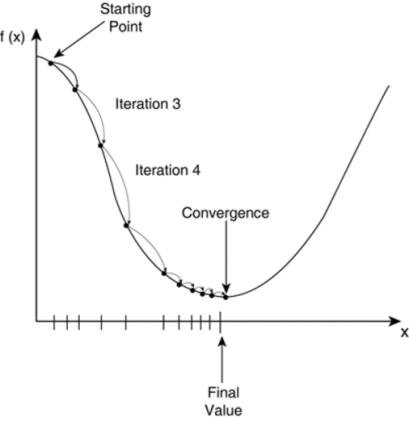
\includegraphics[width=\textwidth]{Sources/03-01_2_dimensionale_grafik_gd.png}
        \caption{2-dimensionaler Gradientenabstieg}
        \label{subsec:2-dimensionaler Gradientenabstieg}
        %TO-DO Quellennachweise einfügen(Abbildungsverzeichnis)
    \end{minipage}\hfill
    \begin{minipage}{0.45\textwidth}
        \centering
        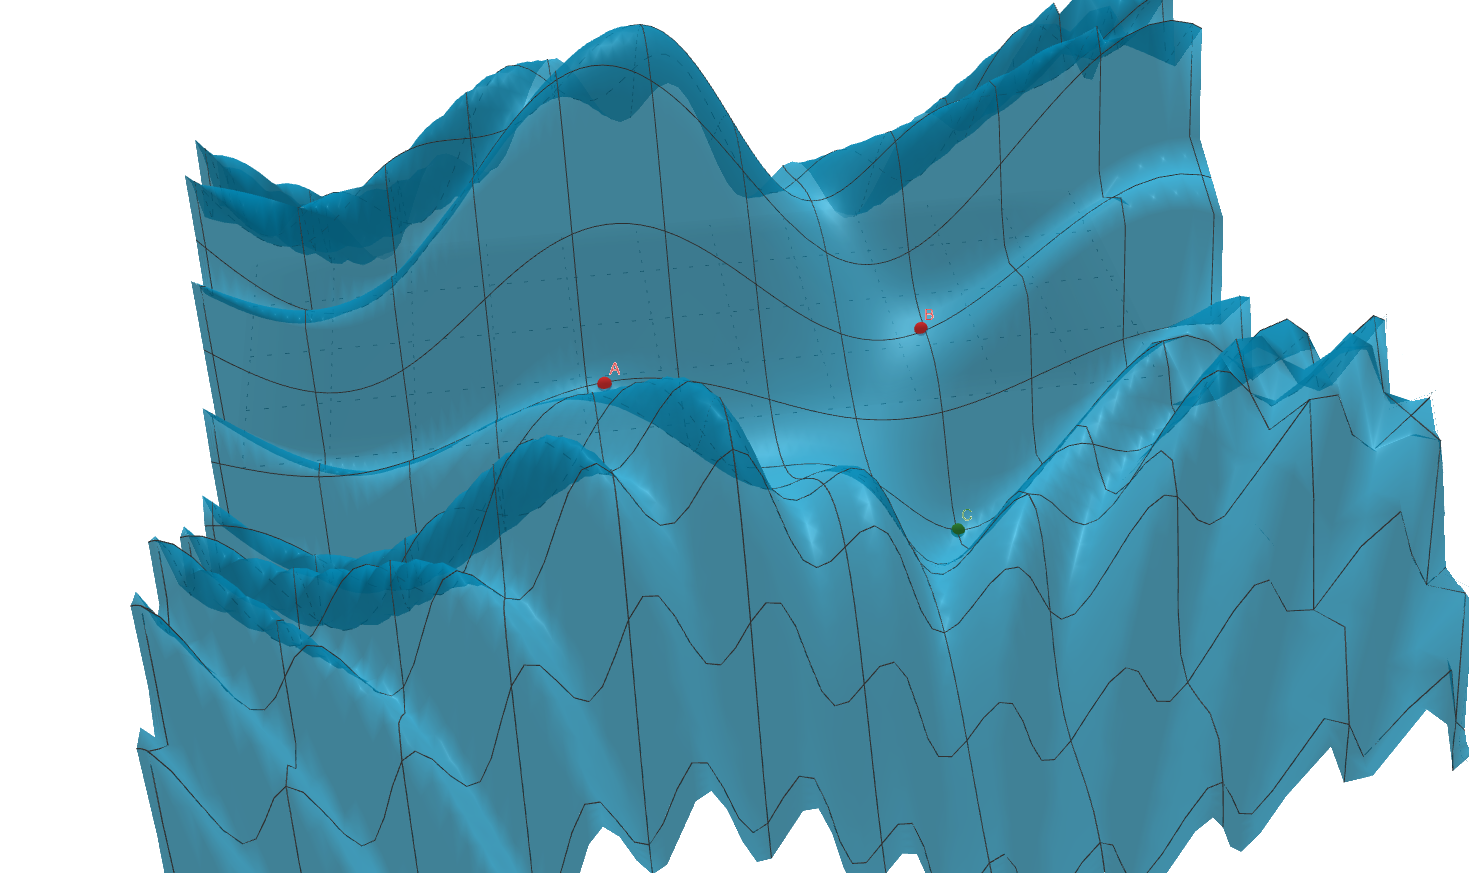
\includegraphics[width=\textwidth]{Sources/03-3.2.3_geogebra.png}
        \caption{3-dimensionaler Gradientenabstieg}
        \label{subsec:3-dimensionaler Gradientenabstieg}
        %TO-DO Quellennachweise einfügen(Abbildungsverzeichnis)
    \end{minipage}
\end{figure}
\newpage
 'Mathematisch ist der steilste Abstieg druch den sogenannten Gradienten(daher der Name Gradientenverfahren) repräsentiert bzw. genauer gesagt durch den negativen Gradienten, da der 
  Gradient selbst den stärksten Anstieg in der 'Hügellandschaft' makiert. Der Gradient gibt nicht nur die Richtung, sondern zugleich auch die Steigung des 'Hügels', sowie stellt folglich
  einen n-1-dimensionalen Vektor dar'\cite{GR10}.
\fi
\subsection{Gefährliche Fehlerquellen}\label{subsec:gradientenverfahren:fehlerquellen}
\subsubsection{Steckt man in einem lokalen Minimum fest?}\label{subsec:gradientenverfahren:fehlerquellen_lokalen_minimum}
  %\input{}
  Auf der Suche nach dem globalen Minimum, kann der Algorithmus in einem lokalen Minimum enden und somit das erreichen des globalen Minimums verhindert werden.
  Ein lokales Minimum tritt auf, wenn das Netzwerk in einem Punkt des Fehlergradienten auf eine niedrigere Fehlerfunktionsebene trifft, aber in der Nähe dieses Punktes einen anderen Punkt mit noch niedrigerem Fehler existiert(siehe Abb.4).
  Da Neuronale Netze häufig große Anzahlen von Parametern haben, kann die Suche nach dem globalen Minimum eine schwierige Aufgabe sein\cite{HS97}.
  \\
  \begin{figure}[ht]
    \centering
    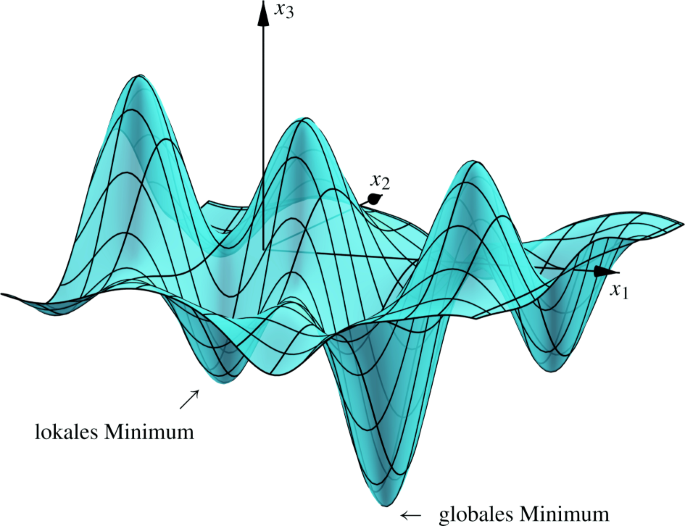
\includegraphics[width=0.5\textwidth]{Sources/03-3.3.2_3-dimensionaler_abstieg.png}
    \caption{Lokales und Global Minimum}
    \label{subsec:lokale-globale-minima}
\end{figure}

\subsubsection{Befindet man sich wirklich im globalen Minimum?}\label{subsec:gradientenverfahren:fehlerquellen_globalen_minimum}
  %\input{}
  Gradientenabstiegs- und Suchverfahren finden in der Regel nur lokale Minima, abhängig vom gewählten Startpunkt. Durch die fehlende Kenntnis der gesamten n-dimensionalen 'Hügellandschaft', die sich hinter 
  einem 'Nebelschleier' verbirgt, ist de facto nie, (ausgenommen der gesamte Fehlerterm liegt bei Null (In diesem Fall ist gewährleistet, das es sich um ein globales Minimum handelt))
  sichergestellt, dass das Verfahren das 'tiefte Tal' -d.h. das globale Minimum - findet.

\subsubsection{Wie löst man dieses Problem?}\label{subsec:gradientenverfahren:fehlerquellen_problem_loesen}
Es stehen zahlreiche Möglichkeiten zue Effizienzsteigerung des Gradientabstiegsverfahren zu Verfügung das Gradientenverfahren um weitere Techniken oder Variationen zu erweitern.
\begin{itemize}
  \item Initialisierung der Gewichte verändern:\\
  Man kann versuchen. die Initialisierung der Gewichte zu verändern, um den Lernerfolg zu verbessern. Dabei ist zu beachten, das sowohl die Art der Initialisierung für das Auffinden eine lokalen bzw. globalen 
  Minimums von Bedeutung ist, als auch der Startpunkt des Gradientabstiegsverfahren, welcher einen zentralen Einfluss darauf hat, welche Werte die Gewichte im Verlauf des Verfahrens annehmen und ob sich ein Lokales
  oder globales Mimimum findet.\\
  Die Initialisierung aller Gewichte auf denselben Zahlenwert führt dazu, das die Gewichte das die Gewichte in der Traininngsphase gleich verändert werden. Um diesem Problem zu begegnen wird die Initialisierung
  der Gewichte mit kleinen, um Null herum streuenden Zufallsgewichten vorgenommen(symmetry breaking). häufig kommt das sogenannte "Multi-Start-Verfahren" zum Einsatz, bei dem die Berechnungen mit verschiedenen
  Startpunkten wiederholt werden. 
\end{itemize}
\begin{itemize}
  \item Lernparameter verändern:\\
  Neben Neu-Initialisierung kann der Lernparameter erhöht werden. Das erhöhen des Lernparameters bewirkt größere Sprünge zum Mimimum. Vorteil dabei ist, das flache Plateaus schneller durchlaufen
  werden. Beim reduzieren des Lernparameters ergibt sich der Vorteil, das das globale Minimum nichtmehr so leicht übersprungen werden kann. Ein Nachteil dabei wäre, das das trainieren eine inakzeptable
  lange Traininngszeiut erreicht.\\
  "Eine weitere Möglichkeit besteht in der stufenweisen Veränderung der Lernrate im Verlauf der Traininngsphase. Genauer gesagt wie der Lernparameter im laufe des Training forlaufend reduziert wird"\cite[Seite 46]{GR10}.\\
\end{itemize}
\begin{itemize}
  \item Momentum-Term inzufügen:\\
  "Der Momentum-Term addiert zum aktuellen Gradienten den vorangegangenen Gradienten. Dieser "vorangegangene" Gradient wird mit dem Momentum-Parameter $\alpha$ multipliziert(Macho,2002) um zu gewährleisten, das dieser nicht
  in der gleichen Stärke wie der aktuelle Gradient die neue Gewichtsveränderungen beinflusst. Stellt man sich das Gradientabstiegsverfahren als ein BHall vor, der eine Hügellandschaft herunterrollt
  bzw. herunterspringt, dann erfolgen die Richtungsveränderungen diesen Ball "Schwung" und kann somit Beispielweise ein flaches Plateau besser überwinden." Folgende Vortile sind mit dem Momentum-Term verknüpft:\\
  \begin{itemize}
  \item Lokale Minima werden eher übersprungen
  \item Flache Plateaus werden aufgrund der Beschleunigung schneller durchlaufen.
  \item Jedoch birgt sein Einsatz auch die erhöhte Gefahr des Überspringen des globalen Minimums.
  \end{itemize}
\end{itemize}
\begin{itemize}
  \item  Delta-Bar-Delta-Regel:\\
  Bei dieser Regel wird ein Vergleich der partiellen Ableitung aus allen aufeinanderfolgenden Durchgänge vorgenommen. Dabei werden auch weit zurückliegende partielle Ableitungen aufgrund eines Gewichtsfaktors 
  berücksichtigt. In Abhängigkeit des Ergebnisses des Vergleichs wird die aktuelle Schrittweite erhöht oder reduziert.\\
\end{itemize}
Trotz der Zahlreichen Lösungsansätze zur Problemstellung, die mit der Kenntnis lediglich der lokalen Umgebung der n-dimensionalen "Gebirgslandschaft" einhergehen, ist keine der Lösungen bei sämtlichen Problemen 
von Vorteil. Stattdessen ist oft simples ausprobieren notwendig, um die geeigneten Ansätze und Parameter auszuwählen\cite[Seite 48]{GR10}.



